\documentclass[tikz,border=6pt]{standalone}
\usepackage[T1]{fontenc}
\usepackage{helvet}
\renewcommand{\familydefault}{\sfdefault}
\usetikzlibrary{positioning,arrows.meta,calc,fit,shapes.geometric,shapes.misc,shapes.multipart}
\newcommand{\dt}{\,\textperiodcentered\,}
\tikzset{
  arr/.style={-{Latex[length=2.2mm]},line width=0.6pt},
  darr/.style={{Latex[length=2.2mm]}-{Latex[length=2.2mm]},line width=0.6pt},
  dashedarr/.style={-{Latex[length=2.2mm,open]},line width=0.6pt,dashed},
  retarr/.style={-{Latex[length=2.2mm]},line width=0.6pt,dashed},
  lbl/.style={font=\footnotesize\itshape},
}

\begin{document}
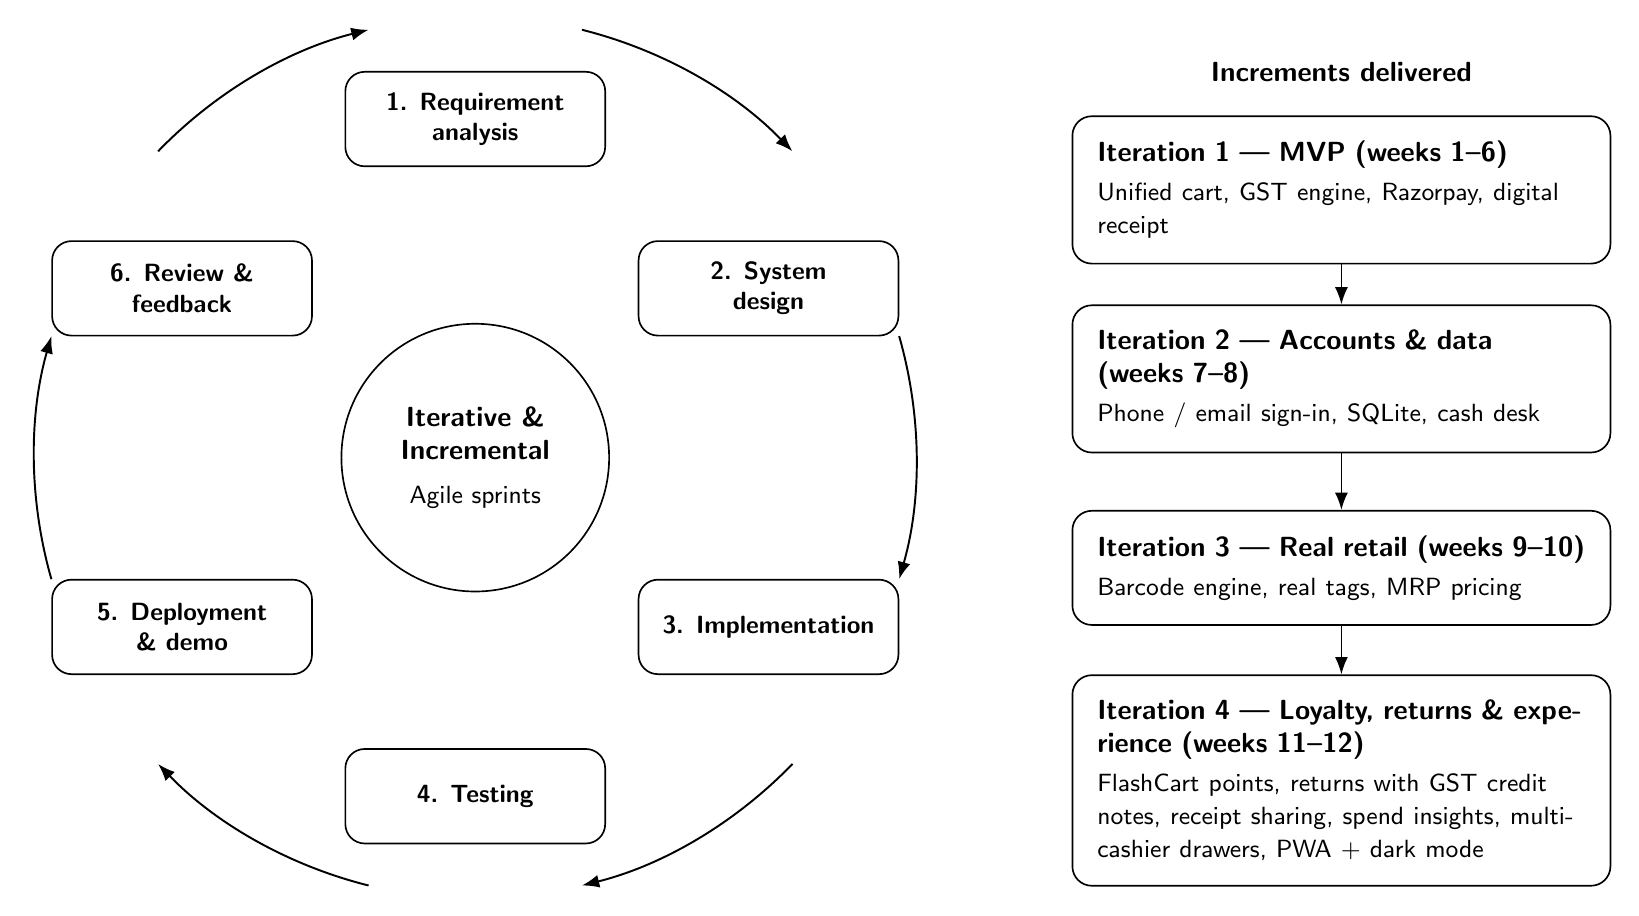
\begin{tikzpicture}[
  ph/.style={draw,rounded corners=7pt,align=center,font=\small\bfseries,inner sep=6pt,minimum width=3.3cm,minimum height=1.2cm,line width=0.6pt},
  it/.style={draw,rounded corners=7pt,align=left,inner sep=9pt,text width=6.2cm,line width=0.6pt},
  curve/.style={arr,line width=0.7pt}]
\def\Rr{4.3}\def\Ra{5.6}
\foreach \i/\txt in {0/1. Requirement\\analysis, 1/2. System\\design, 2/3. Implementation, 3/4. Testing, 4/5. Deployment\\\& demo, 5/6. Review \&\\feedback} {
  \node[ph] (p\i) at (90-\i*60:\Rr) {\txt};
}
\foreach \i in {0,...,5} {
  \draw[curve] ($(90-\i*60-14:\Ra)$) arc (90-\i*60-14:90-\i*60-46:\Ra);
}
\node[draw,circle,minimum size=3.4cm,align=center,line width=0.6pt] at (0,0) {\bfseries Iterative \&\\\bfseries Incremental\\[4pt]\small Agile sprints};
% increments
\node[font=\bfseries] at (11.0,4.9) {Increments delivered};
\node[it] (i1) at (11.0,3.4) {\textbf{Iteration 1 --- MVP (weeks 1--6)}\\[2pt]\small Unified cart, GST engine, Razorpay, digital receipt};
\node[it] (i2) at (11.0,1.0) {\textbf{Iteration 2 --- Accounts \& data (weeks 7--8)}\\[2pt]\small Phone / email sign-in, SQLite, cash desk};
\node[it] (i3) at (11.0,-1.4) {\textbf{Iteration 3 --- Real retail (weeks 9--10)}\\[2pt]\small Barcode engine, real tags, MRP pricing};
\node[it] (i4) at (11.0,-4.1) {\textbf{Iteration 4 --- Loyalty, returns \& experience (weeks 11--12)}\\[2pt]\small FlashCart points, returns with GST credit notes, receipt sharing, spend insights, multi-cashier drawers, PWA + dark mode};
\draw[arr] (i1) -- (i2);
\draw[arr] (i2) -- (i3);
\draw[arr] (i3) -- (i4);
\end{tikzpicture}
\end{document}
